\chapter{\label{ch:3}Measuring nucleotide binding to K\ATP} 

\graphicspath{{figures/ch3/}}

\minitoc

\section{Choosing a site to incorporate Anap}

Needs to fulfill a number of criteria:

Close enough to the binding site to measure FRET.
Far enough from other classes of binding site to avoid inteference.
Far enough from other subunits to avoid cross talk.

\begin{figure}[h]
	\centering
	\begin{subfigure}[t]{0.4\textwidth}
		\caption{}\label{ch3fig:chemical_structures}
		\centering
		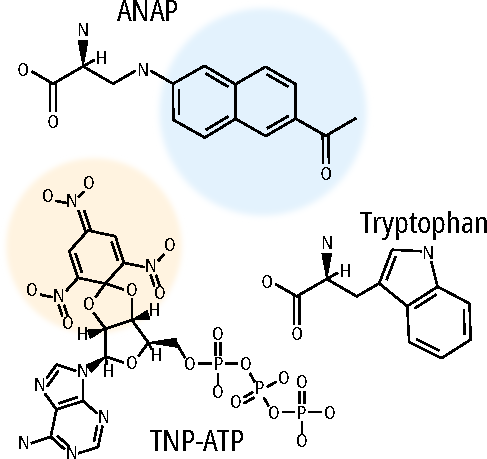
\includegraphics[width=\textwidth]{chemical_structures.pdf}
	\end{subfigure}
	\hfill
	\parbox[t]{0.5\textwidth}{
	\begin{subfigure}[t]{0.5\textwidth}
		\caption{}\label{ch3fig:spectral_overlap}
		\centering
		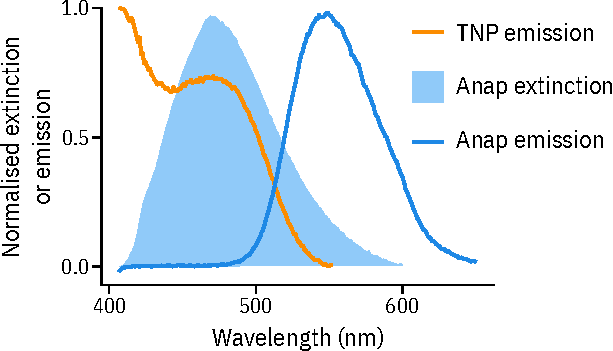
\includegraphics[width=\textwidth]{spectral_overlap.pdf}
	\end{subfigure}
	\hfill
	\begin{subfigure}[t]{0.5\textwidth}
		\caption{}\label{ch3fig:fret_efficiency}
		\centering
		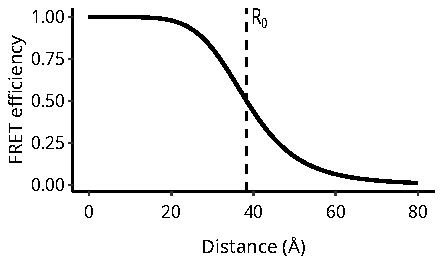
\includegraphics[width=\textwidth]{fret_efficiency.pdf}
	\end{subfigure}
	}
	\caption[Anap and TNP-nucleotides as FRET pairs]{
		\subref{ch3fig:chemical_structures} Chemical structures of Anap and TNP-ATP shown with the fluorescent moieties highlighted in blue (Anap) ot ornage (TNP-ATP).
		\subref{ch3fig:spectral_overlap} Normalised emission spectra (solid lines) of Anap (blue) and TNP-nucleotides (orange) overlayed on the normalised extinction spectra of Anap (filled light blue area).
		Extinction spectra were measured from Anap and TNP-nucleotides alone in aqueous solution.
		Anap emission is the averaged spectra from Kir6.2* + SUR1 expressed in unroofed membranes.
		\subref{ch3fig:fret_efficiency} Theoretical FRET efficiency displayed as a function of the distance between donor and acceptor fluorophores.
		The curve was calculated as a function of the overlap shown in \subref{ch3fig:spectral_overlap}.
		The full formula is discussed in Chapter \ref{ch:2-methods}.
	}

\end{figure}



\subsection{Scanning a region}

Introduced cutting sites and pasted in oligos
(with Mike and Tascia - Mike did the molecular biology on SUR, I did on Kir6.2, Mike and I did surface expression together, Tascia did ephys on the mutants that expressed).

\subsection{Rational residues}

Number of hydrophobic residues chosen and mutated.
Checked with exiFret v2 (might put discussion of this in appendix)

\section{Testing for membrane expression}

\subsection{Expression with SUR1}

Surface expression assay

Confocal microscopy

Electrophys

\subsection{Expression alone/with TMD0(195/232)}

Surface expression assay

Confocal (not with TMD0s)

Electrophys (tolbutamide)